\renewcommand{\theequation}{\theenumi}
\begin{enumerate}[label=\arabic*.,ref=\thesubsection.\theenumi]
\numberwithin{equation}{enumi}
\item The area of triangle $ABC$: \\
\solution The area of triangle $ABC$ using cross product is obtained as:
\begin{align}
\frac{1}{2}\norm{(\vec{B}-\vec{A})\times(\vec{C}-\vec{A})}
\\
\frac{1}{2}\norm{(\myvec{-3\\-5}-\myvec{-4\\2})\times(\myvec{3\\-2}-\myvec{-4\\2})}
\\
\frac{1}{2}\norm{\myvec{1\\-7} \times \myvec{7\\-4}} = \frac{45}{2}
\end{align}
Area of $\triangle{ABC}$ = $22.5 units^2$
and it is found in the following python code:
\begin{lstlisting}
codes/tri_area_ABC.py
\end{lstlisting} 

\item The area of triangle $ACD$: \\
\solution The area of triangle $ACD$ using Heron's formula is obtained as:
\begin{align}
\frac{1}{2}\norm{(\vec{C}-\vec{A})\times(\vec{D}-\vec{A})}
\\
\frac{1}{2}\norm{(\myvec{3\\-2}-\myvec{-4\\2})\times(\myvec{2\\3}-\myvec{-4\\2})}
\\
\frac{1}{2}\norm{\myvec{7\\-4} \times \myvec{6\\1}} = \frac{31}{2}
\end{align}
Area of $\triangle{ACD}$ = $15.5 units^2$
and it is found in the following python code:
\begin{lstlisting}
codes/tri_area_ACD.py
\end{lstlisting} 

\item The area of quadrilateral $ABCD$: \\
\solution Area of Quadrilateral $ABCD$ = Area of $\triangle{ABC}$ + Area of $\triangle{ACD}$ = $38 units^2$ 

\item Quadrilateral $ABCD$ in Fig.\ref{fig:quad_1} is generated using the following python code 
\begin{lstlisting}
codes/quadrilateral/quad.py
\end{lstlisting}
\begin{figure}[!ht]
\centering
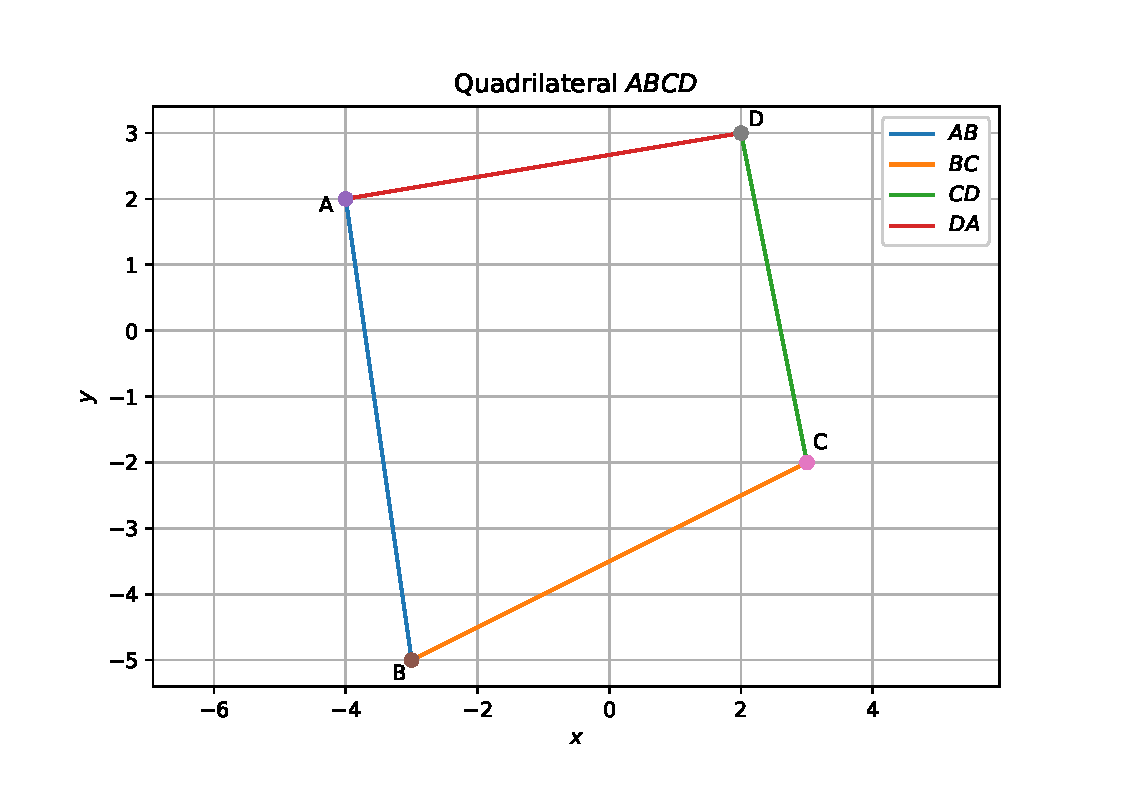
\includegraphics[width=\columnwidth]{./codes/quadrilateral/quad.eps}
\caption{Quadrilateral $ABCD$ using python}
\label{fig:quad_1}
\end{figure} 
\end{enumerate}